\documentclass{article}

% PACKAGES
\usepackage[margin=0.75in]{geometry}
\usepackage{amsmath}
\usepackage{amssymb}
\usepackage{graphicx}
\usepackage{subcaption}
\usepackage{hyperref}
\usepackage{wrapfig}

\title{ECE 269 - Final Project Report\\Orthogonal Matching Pursuit}
\author{Eric Weise}
\date{December 17, 2020}

\begin{document}

\maketitle

My project is hosted on GitHub:

\url{https://github.com/ericdweise/ece269/blob/master/report.pdf}




\section*{Background}











%%%%%%%%%%%%%%%%%%
%%%   PART C   %%%
%%%%%%%%%%%%%%%%%%

\newpage

\section*{Noiseless Signal Recovery ({\it part c})}


\begin{figure}[H]
    \captionsetup{width=.75\linewidth}
    \centering
        \includegraphics[width=0.25\textwidth]{plots/c-recov_N-20.png}
        \includegraphics[width=0.25\textwidth]{plots/c-recov_N-50.png}
        \includegraphics[width=0.25\textwidth]{plots/c-recov_N-100.png}
        \newline
        \includegraphics[width=0.25\textwidth]{plots/c-error_N-20.png}
        \includegraphics[width=0.25\textwidth]{plots/c-error_N-50.png}
        \includegraphics[width=0.25\textwidth]{plots/c-error_N-100.png}
        \caption{Noiseless support set recovery. Top row: The probability of Exact Support Recovery. Bottom row: Normalized error of recovered signal. NOTE: The ESR and the error plots are viewed from different angles.}
\end{figure}

The Exact Signal Recovery (ESR) rate is very highly correlated to s, and somewhat correlated to M.
This is evident in the sharp 

The Normalized Error plots show roughtly the inverse trend as that in the ESR plots:
The Error rate is low for small sparsity, and reach a plateau close to 1.2.















%%%%%%%%%%%%%%%%%%%
%%%   PART D1   %%%
%%%%%%%%%%%%%%%%%%%

\newpage
\section*{Noisy Signal Recovery With Known Sparsity ({\it Part d-i})}


\begin{figure}[H]
    \captionsetup{width=.75\linewidth}
    \centering
        \includegraphics[width=0.25\textwidth]{plots/d1-recov_N-20_noise-0.05.png}
        \includegraphics[width=0.25\textwidth]{plots/d1-recov_N-50_noise-0.05.png}
        \includegraphics[width=0.25\textwidth]{plots/d1-recov_N-100_noise-0.05.png}
        \newline
        \includegraphics[width=0.25\textwidth]{plots/d1-error_N-20_noise-0.05.png}
        \includegraphics[width=0.25\textwidth]{plots/d1-error_N-50_noise-0.05.png}
        \includegraphics[width=0.25\textwidth]{plots/d1-error_N-100_noise-0.05.png}
        \caption{Noisy support set recovery {\bf variance=0.05}. Stop condition achieved when loop count is the sparsity of the input signal. Top row: The probability of Exact Support Recovery. Bottom row: Normalized error of recovered signal.}
\end{figure}


\begin{figure}[H]
    \captionsetup{width=.75\linewidth}
    \centering
        \includegraphics[width=0.25\textwidth]{plots/d1-recov_N-20_noise-1.png}
        \includegraphics[width=0.25\textwidth]{plots/d1-recov_N-50_noise-1.png}
        \includegraphics[width=0.25\textwidth]{plots/d1-recov_N-100_noise-1.png}
        \newline
        \includegraphics[width=0.25\textwidth]{plots/d1-error_N-20_noise-1.png}
        \includegraphics[width=0.25\textwidth]{plots/d1-error_N-50_noise-1.png}
        \includegraphics[width=0.25\textwidth]{plots/d1-error_N-100_noise-1.png}
        \caption{Noisy support set recovery {\bf variance=1}. Stop condition achieved when loop count is the sparsity of the input signal. Top row: The probability of Exact Support Recovery. Bottom row: Normalized error of recovered signal.}
\end{figure}


As we might predict, adding small amounts of noise changes the ESR and Normalized Error plots slightly, while adding more noise washes out the lots more significantly.















%%%%%%%%%%%%%%%%%%%
%%%   PART D2   %%%
%%%%%%%%%%%%%%%%%%%

\newpage
\section*{Noisy Signal Recovery ({\it part d-ii})}


\begin{figure}[H]
    \captionsetup{width=.75\linewidth}
    \centering
        \includegraphics[width=0.25\textwidth]{plots/d2-recov_N-20_noise-0.05.png}
        \includegraphics[width=0.25\textwidth]{plots/d2-recov_N-50_noise-0.05.png}
        \includegraphics[width=0.25\textwidth]{plots/d2-recov_N-100_noise-0.05.png}
        \newline
        \includegraphics[width=0.25\textwidth]{plots/d2-error_N-20_noise-0.05.png}
        \includegraphics[width=0.25\textwidth]{plots/d2-error_N-50_noise-0.05.png}
        \includegraphics[width=0.25\textwidth]{plots/d2-error_N-100_noise-0.05.png}
        \caption{Noisy support set recovery {\bf variance=0.05}. Stop condition achieved when the 2-norm of residual is less than 0.001. Top row: The probability of Exact Support Recovery. Bottom row: Normalized error of recovered signal.}
\end{figure}


\begin{figure}[H]
    \captionsetup{width=.75\linewidth}
    \centering
        \includegraphics[width=0.25\textwidth]{plots/d2-recov_N-20_noise-1.png}
        \includegraphics[width=0.25\textwidth]{plots/d2-recov_N-50_noise-1.png}
        \includegraphics[width=0.25\textwidth]{plots/d2-recov_N-100_noise-1.png}
        \newline
        \includegraphics[width=0.25\textwidth]{plots/d2-error_N-20_noise-1.png}
        \includegraphics[width=0.25\textwidth]{plots/d2-error_N-50_noise-1.png}
        \includegraphics[width=0.25\textwidth]{plots/d2-error_N-100_noise-1.png}
        \caption{Noisy support set recovery {\bf variance=1}. Stop condition achieved when the 2-norm of residual is less than 0.001. Top row: The probability of Exact Support Recovery. Bottom row: Normalized error of recovered signal.}
\end{figure}















%%%%%%%%%%%%%%%%%%%
%%%   PART D3   %%%
%%%%%%%%%%%%%%%%%%%

\newpage
\section*{Image Recovery ({\it Part d-iii})}

\subsection*{Compressive Sampling and Signal Recovery Methods}

Compressive sensing is a rich field.
The goal is to take the fewest number of samples and maintain recoverability of the source signal.
First we must find an appropriate orthonormal basis ${\psi_1, \ldots, \psi_N}$.
A signal $x$ can be created as a linear combination of the elements $\psi_i$.
Next, a random Gaussian matrix is created, $\Phi \in \mathbb{R}^{M \times N}$ with $M<<N$.
Then, a compressed vector $y$ can be created via:
\begin{align}
    y = \Phi \Psi x
\end{align}
Where the columns of $Psi$ are the orthonormal vectors $\psi_i$.

The purpose of this experiment is to demonstrate the recoverability of a compressed image.
The image will be compressed using equation 1 then recovered using Orthogonal Matching Pursuit.


These are the steps used in Compressive Sensing and Signal Reconstruction.

\begin{enumerate}
    \item First, a random gaussian matrix matrix is made, $\Phi \in \mathbb{R}^{M \times 64}$.
        This is the measurement matrix.
    \item The image is broken into $8 \times 8$ subimages.
        Each sub image will be processed Compressed then recovered.
    \item Each sub image is transformed into frequency space using a Discrete Cosine Transform.
        The $64 \times 64$ DCT matrix forms $\Psi$.
    \item The transformed $8 \times 8$ subimage is converted into a vector $x \in \mathbb{R}^{1 \times 64}$
        The order uses the zig-zag pattern demonstrated in {\it figure 6 to bias low frequency coefficients in Fourier space.
    \item The largest $s$ elements in $x$ are retained. The rest are set to zero. This sparse vector is denoted $x_s$
    \item {\bf Compressive Sensing}: Calculate $y = \Phi \cdot x_s$. ($y \in \mathbb{R}^M$)
    \item Perform OMP to recover $\hat{x} \in \mathbb{R}^{64}$.
        The stop condition is set to $||A\cdot \hat{x} - y||_2 < 10^{-3}$
    \item $\hat{x}$ is converted to an $8 \times 8$ array using the zig-zag ordering.
    \item The Inverse Discrete Cosine Transform is applied to convert the recovered subimage back to image space.
\end{enumerate}

In the above steps $y = \Phi \Psi x$ is the result of compressive sensing.
This process is repeated for every $8 \times 8$ subimage.

\begin{figure}[H]
    \captionsetup{width=.5\linewidth}
    \centering
        \includegraphics[width=0.5\textwidth]{assets/zigzag.jpg}
        \caption{The Zig-zag ordering. In the DCT Basis this preferences low frequency components over higher frequency components.}
\end{figure}


\newpage
\subsection*{Image Recovery After Compressive Sensing}

This experiment was performed on four images.
The imags were chosen to show a varying level of complexity.
The recovered images and some recovered images are shown in figures 7-10.

Even at a very low sparsity level there is significant image reconstruction.
At $s/N = 2/64$ we begin to see some texture, although finer details are not recovered.
However, even at low sparsity levels, around 8, we can see more details being recovered.
Notice the texture in the elephant's skin, the tree branches under the arch, and the hairs of the koala start to appear.

\begin{figure}[H]
    \captionsetup{width=.5\linewidth}
    \centering
        \includegraphics[width=0.25\textwidth]{images/arch.png}
        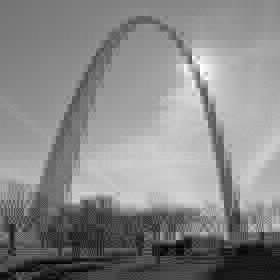
\includegraphics[width=0.25\textwidth]{images/arch-recovered_02.png}
        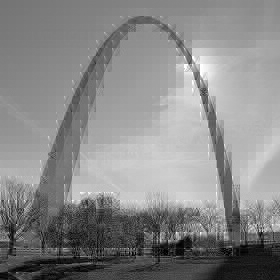
\includegraphics[width=0.25\textwidth]{images/arch-recovered_08.png}
        \caption{The original image of the arch (left) recovered image with s=2 (center) and recovered image with s=8 (right)}
\end{figure}

\begin{figure}[H]
    \captionsetup{width=.5\linewidth}
    \centering
        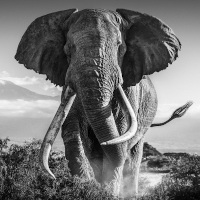
\includegraphics[width=0.25\textwidth]{images/elephant.png}
        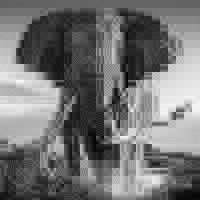
\includegraphics[width=0.25\textwidth]{images/elephant-recovered_02.png}
        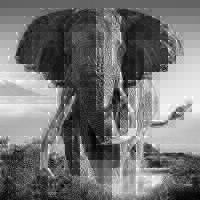
\includegraphics[width=0.25\textwidth]{images/elephant-recovered_08.png}
        \caption{The original image of elephant (left) recovered image with s=2 (center) and recovered image with s=8 (right)}
\end{figure}

\begin{figure}[H]
    \captionsetup{width=.5\linewidth}
    \centering
        \includegraphics[width=0.25\textwidth]{images/koala.png}
        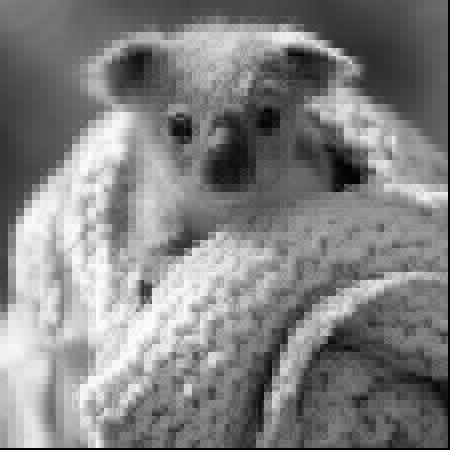
\includegraphics[width=0.25\textwidth]{images/koala-recovered_02.png}
        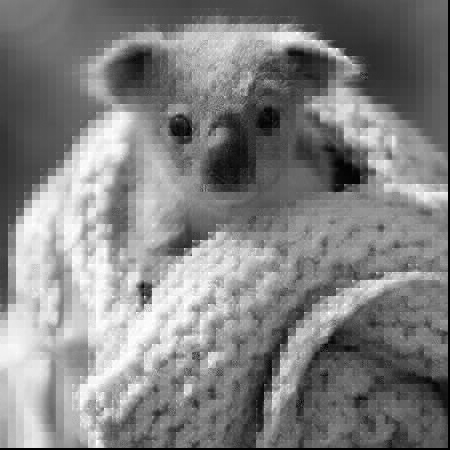
\includegraphics[width=0.25\textwidth]{images/koala-recovered_08.png}
        \caption{The original image of the koala (left) recovered image with s=2 (center) and recovered image with s=8 (right)}
\end{figure}

\begin{figure}[H]
    \captionsetup{width=.5\linewidth}
    \centering
        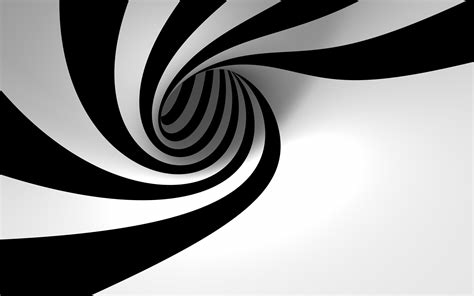
\includegraphics[width=0.25\textwidth]{images/spiral.png}
        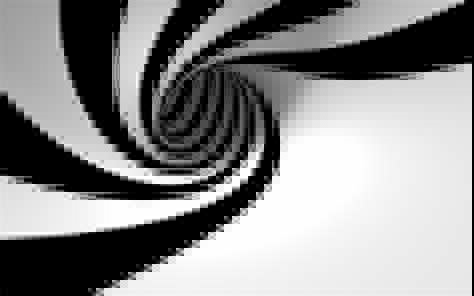
\includegraphics[width=0.25\textwidth]{images/spiral-recovered_02.png}
        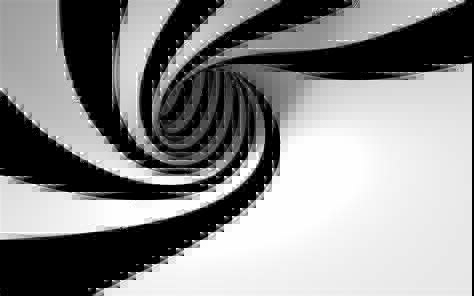
\includegraphics[width=0.25\textwidth]{images/spiral-recovered_08.png}
        \caption{The original image of the spiral (left) recovered image with s=2 (center) and recovered image with s=8 (right)}
\end{figure}



\begin{figure}[H]
    \captionsetup{width=.5\linewidth}
    \centering
        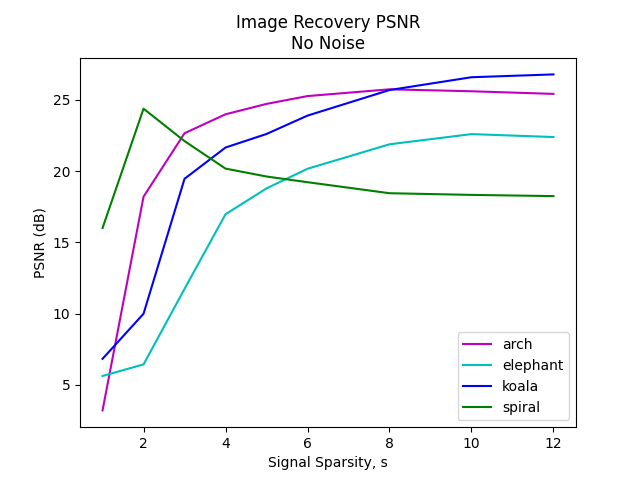
\includegraphics[width=0.5\textwidth]{plots/d3-no-noise.png}
        \caption{PSNR measured for varying sparsity levels and for different levels of added noise.}
\end{figure}




\newpage
\subsection*{Image Recovery With Added Noise}

The process of reconstructing the noisy image is the same as the previous section.
Before the process of compressive sensing begins , however, random noise is added to the image.
Each pixel has a random number drawn from a normal distribution.
This is done twice, first with a variance of 10, then again with a variance of 50.
The mean for both experiments is zero.



\subsubsection*{Variance=10}
\begin{figure}[H]
    \captionsetup{width=.5\linewidth}
    \centering
        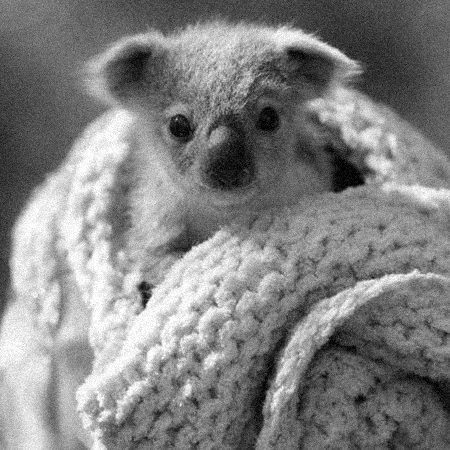
\includegraphics[width=0.25\textwidth]{images/koala_noise-10.png}
        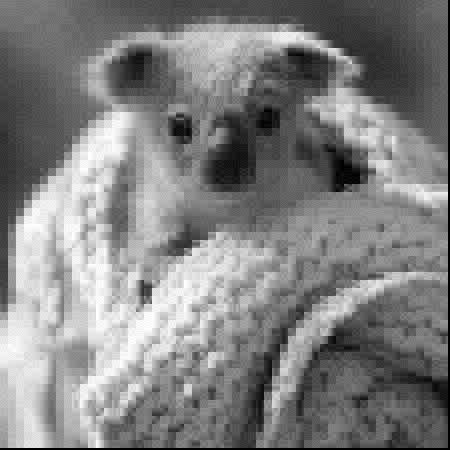
\includegraphics[width=0.25\textwidth]{images/koala_noise-10-recovered_02.png}
        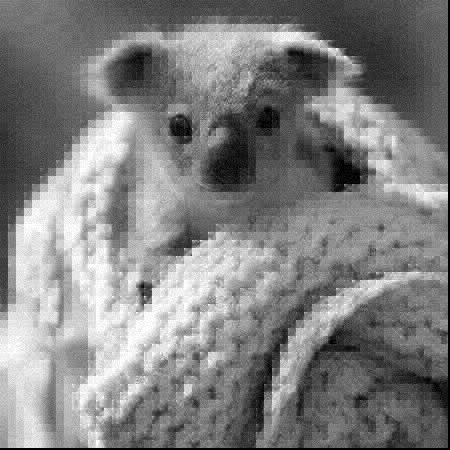
\includegraphics[width=0.25\textwidth]{images/koala_noise-10-recovered_08.png}
        \caption{Results for image reconstruction with added noise {\bf variance=10}. From left to right: Image with added noise. Recovery with sparsity 2. Recovery with sparsity 8.}
\end{figure}


\newpage
\subsubsection*{Variance=50}
\begin{figure}[H]
    \captionsetup{width=.5\linewidth}
    \centering
        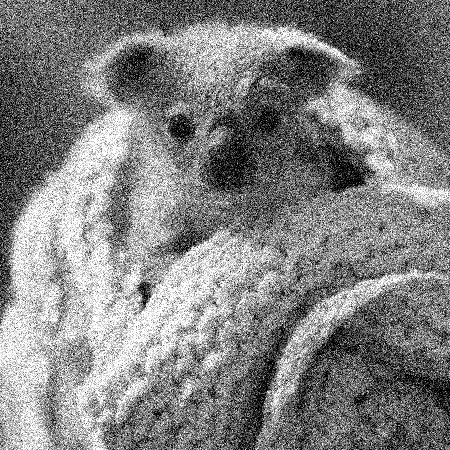
\includegraphics[width=0.25\textwidth]{images/koala_noise-50.png}
        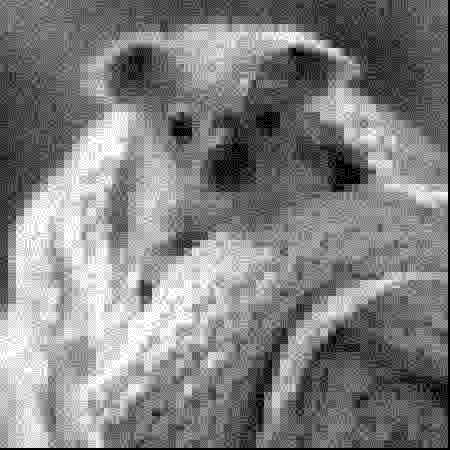
\includegraphics[width=0.25\textwidth]{images/koala_noise-50-recovered_02.png}
        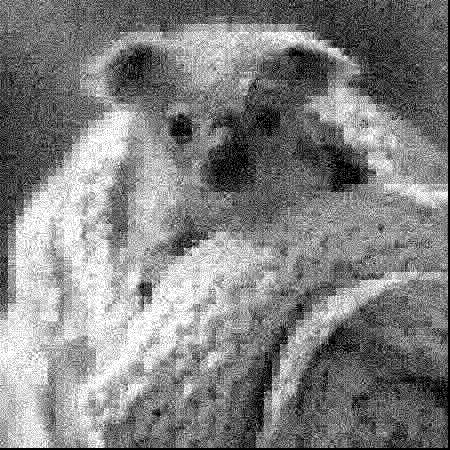
\includegraphics[width=0.25\textwidth]{images/koala_noise-50-recovered_08.png}
        \caption{Results for image reconstruction with added noise {\bf variance=50}. From left to right: Image with added noise. Recovery with sparsity 2. Recovery with sparsity 8.}
\end{figure}


\begin{figure}
    \captionsetup{width=.45\linewidth}
    \centering
        \includegraphics[width=0.45\textwidth]{plots/d3-noise-10.png}
        \includegraphics[width=0.45\textwidth]{plots/d3-noise-50.png}
        \caption{Peak Signal to Noise Ratio as a function of sparsity for noisy images. Top variance=10, bottom variance=50.}
\end{figure}

\end{document}
